\documentclass[11pt]{article}
\usepackage[textwidth=18.0cm, textheight=23.0cm, top=2.0cm]{geometry}
\usepackage{pst-all}
\usepackage{amssymb}
\usepackage{tikz}
\usepackage{underscore}\begin{document}
\pagestyle{empty}


ClassName: \underline{\textbf{Class_03.2bp-1}}
\par
BinSize: \underline{\textbf{40 × 40}}
\par
ReduceSize: \underline{\textbf{40 × 40}}
\par
TypeNum: \underline{\textbf{19}}
\par
Num: \underline{\textbf{20}}
\par
OutS: \underline{\textbf{6400}}
\par
InS: \underline{\textbf{4169}}
\par
Rate: \underline{\textbf{0.651}}
\par
UB: \underline{\textbf{4}}
\par
LB0: \underline{\textbf{3}}
\par
LB: \underline{\textbf{4}}
\par
LBWithCut: \underline{\textbf{4}}
\par
NodeCut: \underline{\textbf{0}}
\par
ExtendedNodeCnt: \underline{\textbf{1}}
\par
GenNodeCnt: \underline{\textbf{1}}
\par
PrimalNode: \underline{\textbf{0}}
\par
ColumnCount: \underline{\textbf{39}}
\par
TotalCutCount: \underline{\textbf{0}}
\par
RootCutCount: \underline{\textbf{0}}
\par
LPSolverCnt: \underline{\textbf{36}}
\par
PricingSolverCnt: \underline{\textbf{36}}
\par
BranchAndBoundNum: \underline{\textbf{1}}
\par
isOpt: \underline{\textbf{true}}
\par
TimeOnInitSolution: \underline{\textbf{600.000 s}}
\par
TimeOnPrimal: \underline{\textbf{0.000 s}}
\par
TimeOnPricing: \underline{\textbf{11.751 s}}
\par
TimeOnRmp: \underline{\textbf{0.124 s}}
\par
TotalTime: \underline{\textbf{612.156 s}}
\par
\newpage


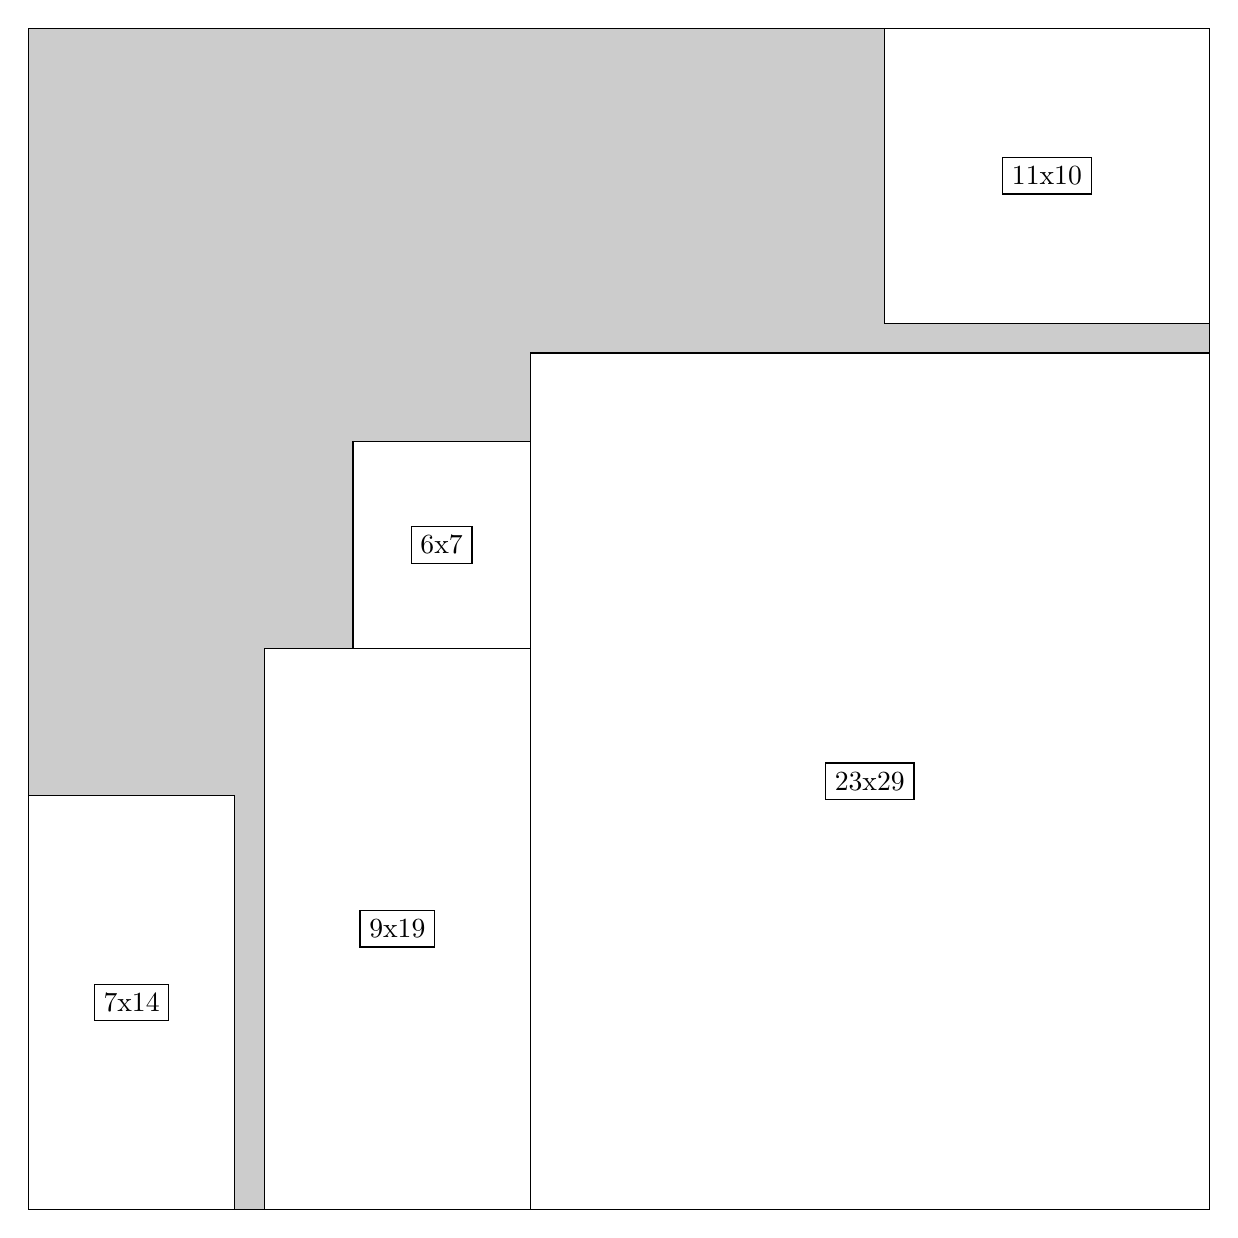
\begin{tikzpicture}[shorten >=1pt,scale=1.0,every node/.style={scale=1.0},->]
\tikzstyle{vertex}=[circle,fill=black!25,minimum size=14pt,inner sep=0pt]
\filldraw[fill=gray!40!white, draw=black] (0,0) rectangle (15.0,15.0);
\foreach \name/\x/\y/\w/\h in {23x29/6.375/0.0/8.625/10.875,9x19/3.0/0.0/3.375/7.125,6x7/4.125/7.125/2.25/2.625,11x10/10.875/11.25/4.125/3.75,7x14/0.0/0.0/2.625/5.25}
\filldraw[fill=white!40!white, draw=black] (\x,\y) rectangle node[draw] (\name) {\name} ++(\w,\h);
\end{tikzpicture}


w =23 , h =29 , x =17 , y =0 , v =667
\par
w =9 , h =19 , x =8 , y =0 , v =171
\par
w =6 , h =7 , x =11 , y =19 , v =42
\par
w =11 , h =10 , x =29 , y =30 , v =110
\par
w =7 , h =14 , x =0 , y =0 , v =98
\par
\newpage


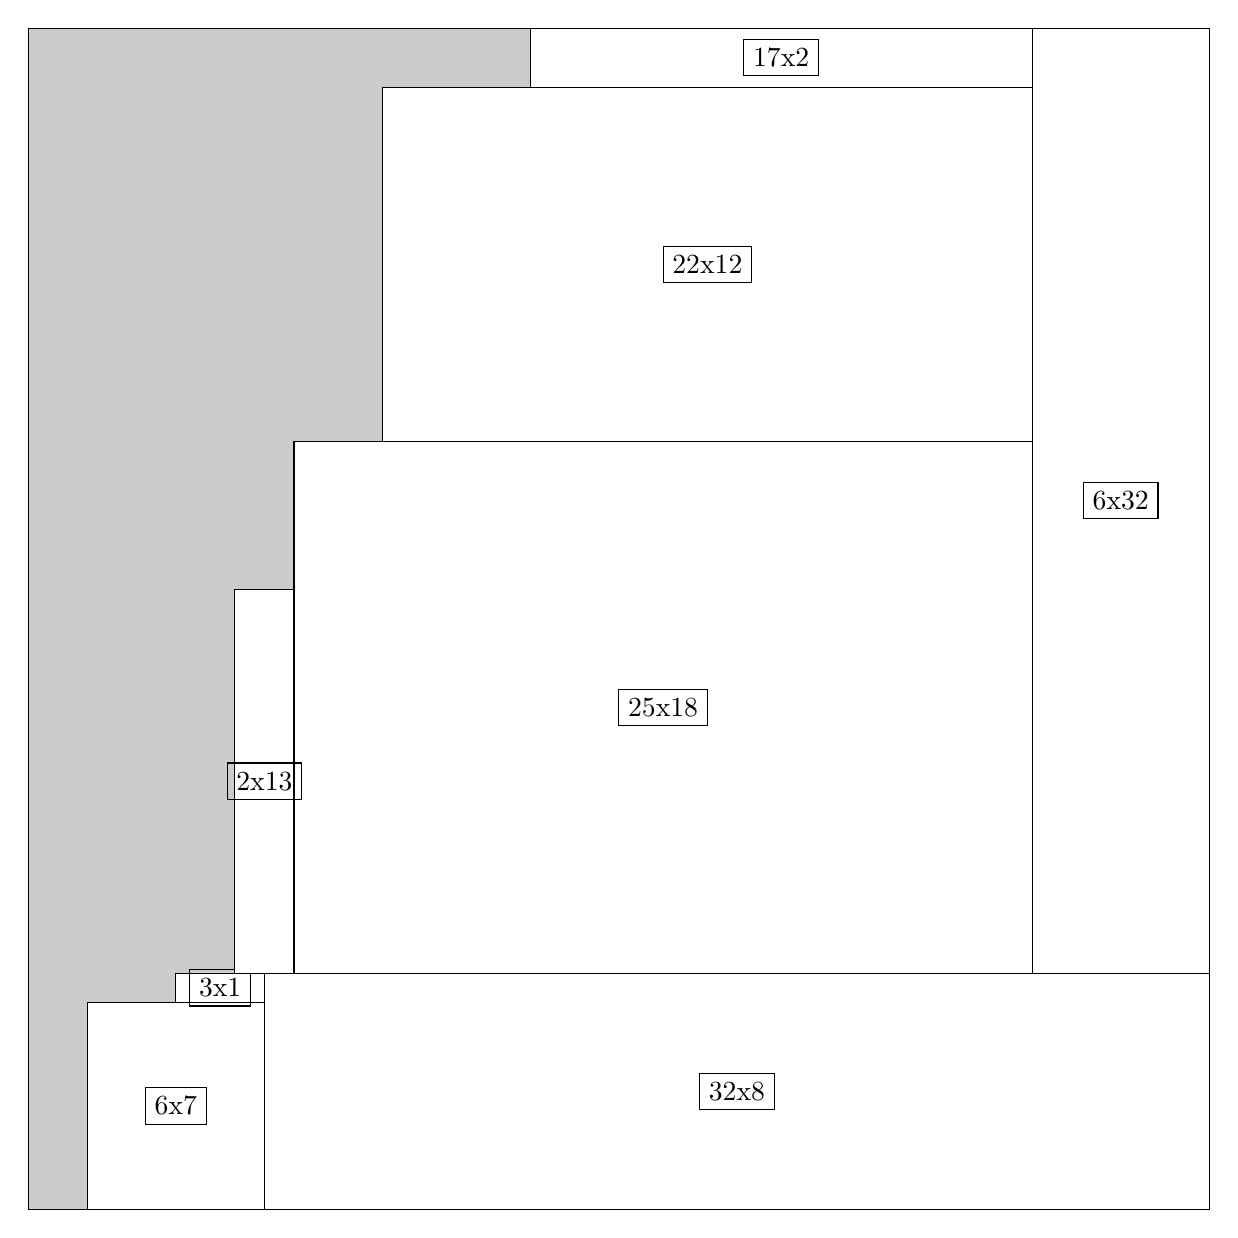
\begin{tikzpicture}[shorten >=1pt,scale=1.0,every node/.style={scale=1.0},->]
\tikzstyle{vertex}=[circle,fill=black!25,minimum size=14pt,inner sep=0pt]
\filldraw[fill=gray!40!white, draw=black] (0,0) rectangle (15.0,15.0);
\foreach \name/\x/\y/\w/\h in {32x8/3.0/0.0/12.0/3.0,6x7/0.75/0.0/2.25/2.625,3x1/1.875/2.625/1.125/0.375,6x32/12.75/3.0/2.25/12.0,25x18/3.375/3.0/9.375/6.75,2x13/2.625/3.0/0.75/4.875,22x12/4.5/9.75/8.25/4.5,17x2/6.375/14.25/6.375/0.75}
\filldraw[fill=white!40!white, draw=black] (\x,\y) rectangle node[draw] (\name) {\name} ++(\w,\h);
\end{tikzpicture}


w =32 , h =8 , x =8 , y =0 , v =256
\par
w =6 , h =7 , x =2 , y =0 , v =42
\par
w =3 , h =1 , x =5 , y =7 , v =3
\par
w =6 , h =32 , x =34 , y =8 , v =192
\par
w =25 , h =18 , x =9 , y =8 , v =450
\par
w =2 , h =13 , x =7 , y =8 , v =26
\par
w =22 , h =12 , x =12 , y =26 , v =264
\par
w =17 , h =2 , x =17 , y =38 , v =34
\par
\newpage


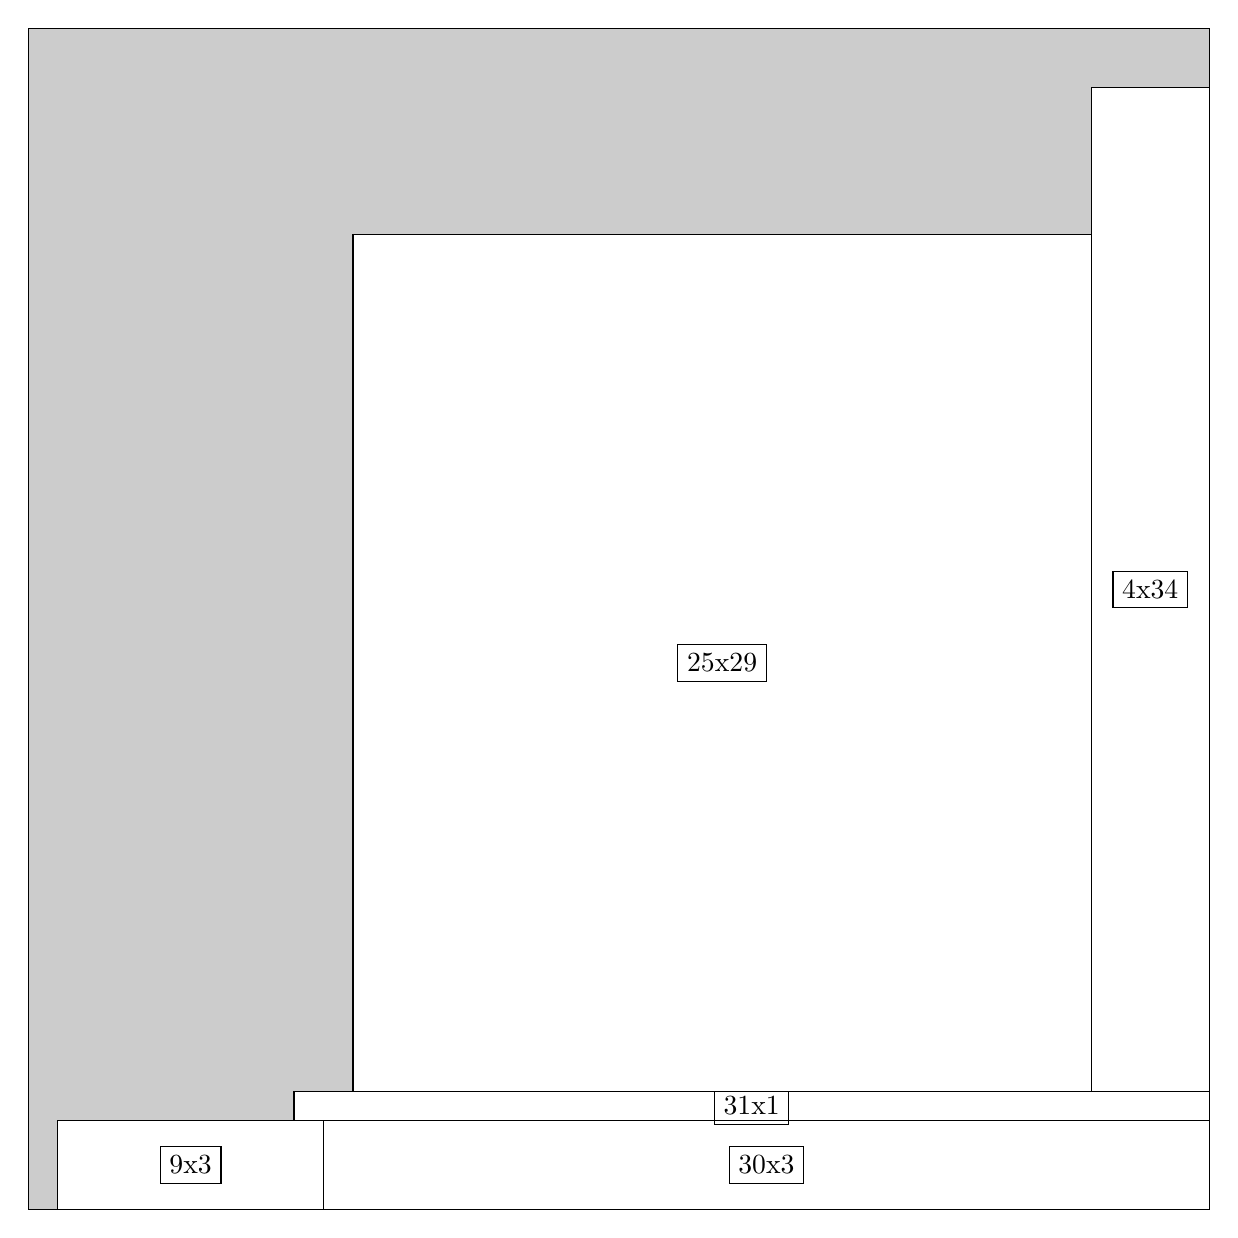
\begin{tikzpicture}[shorten >=1pt,scale=1.0,every node/.style={scale=1.0},->]
\tikzstyle{vertex}=[circle,fill=black!25,minimum size=14pt,inner sep=0pt]
\filldraw[fill=gray!40!white, draw=black] (0,0) rectangle (15.0,15.0);
\foreach \name/\x/\y/\w/\h in {30x3/3.75/0.0/11.25/1.125,9x3/0.375/0.0/3.375/1.125,31x1/3.375/1.125/11.625/0.375,4x34/13.5/1.5/1.5/12.75,25x29/4.125/1.5/9.375/10.875}
\filldraw[fill=white!40!white, draw=black] (\x,\y) rectangle node[draw] (\name) {\name} ++(\w,\h);
\end{tikzpicture}


w =30 , h =3 , x =10 , y =0 , v =90
\par
w =9 , h =3 , x =1 , y =0 , v =27
\par
w =31 , h =1 , x =9 , y =3 , v =31
\par
w =4 , h =34 , x =36 , y =4 , v =136
\par
w =25 , h =29 , x =11 , y =4 , v =725
\par
\newpage


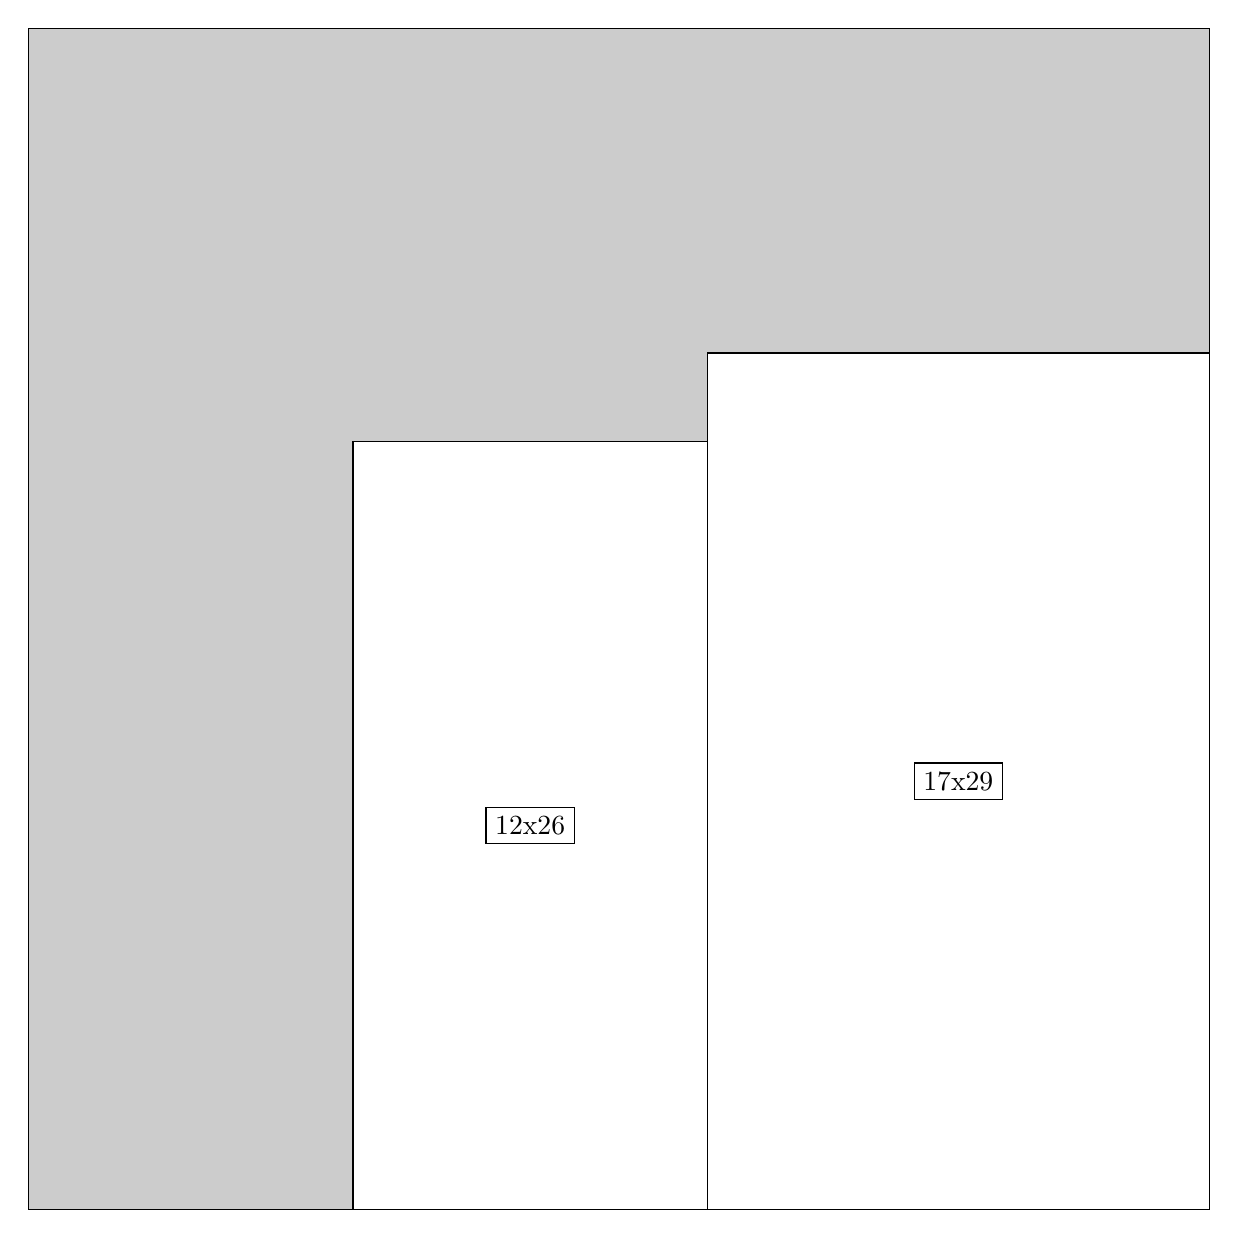
\begin{tikzpicture}[shorten >=1pt,scale=1.0,every node/.style={scale=1.0},->]
\tikzstyle{vertex}=[circle,fill=black!25,minimum size=14pt,inner sep=0pt]
\filldraw[fill=gray!40!white, draw=black] (0,0) rectangle (15.0,15.0);
\foreach \name/\x/\y/\w/\h in {17x29/8.625/0.0/6.375/10.875,12x26/4.125/0.0/4.5/9.75}
\filldraw[fill=white!40!white, draw=black] (\x,\y) rectangle node[draw] (\name) {\name} ++(\w,\h);
\end{tikzpicture}


w =17 , h =29 , x =23 , y =0 , v =493
\par
w =12 , h =26 , x =11 , y =0 , v =312
\par
\newpage


\end{document}